\documentclass{article}
    \title{\textbf{Programación de Sistemas Distribuidos:\\Trabajo Final}}
    \author{Óscar Salvador}
    
	\addtolength{\topmargin}{-2cm}
    \addtolength{\textheight}{3cm}
    \addtolength{\oddsidemargin}{-2cm}
	\addtolength{\textwidth}{4cm}

\usepackage[spanish]{babel}
\usepackage{makeidx}
\usepackage{tikz-cd}

\begin{document}
\maketitle
\clearpage
\tableofcontents


\begin{flushleft}
	\clearpage
	\section{Introducción}
	El sistema está implementado en script de bash, java y python. He utilizado Docker para montar los nodos del sistema. El despliegue implica: compilar el código fuente; instalar el sistema; y ejecutarlo. Estos tres pasos tienen scripts de shell para automatizar el desarrollo y despliegue. Python es usado exclusivamente para aplicar filtros a imagenes. La comunicación está implementada en java. Para los directorios remotos he usado SAMBA, explicaré la razón de esta decisión más adelante.
	
		\subsection{Funcionamiento del sistema}
		El sistema tiene dos versiones, pero solo cambian en los nodos y elementos especificos a cada variante. Los elementos en común son: Cliente; Proxy; Nodo de autenticación; Administrador de Usuarios; y Nodo Central. Hay un CSV con los datos de los usuarios para asegurar la persistencia, este solo es accedido por el nodo de autenticación, y es también común a las dos variantes. El directorio remoto solo aparece en los diagramas de los sistemas, pero es el mismo para los dos.
		\linebreak
		
		\hspace*{2cm}
		\resizebox{0.7\textwidth}{!}{%
			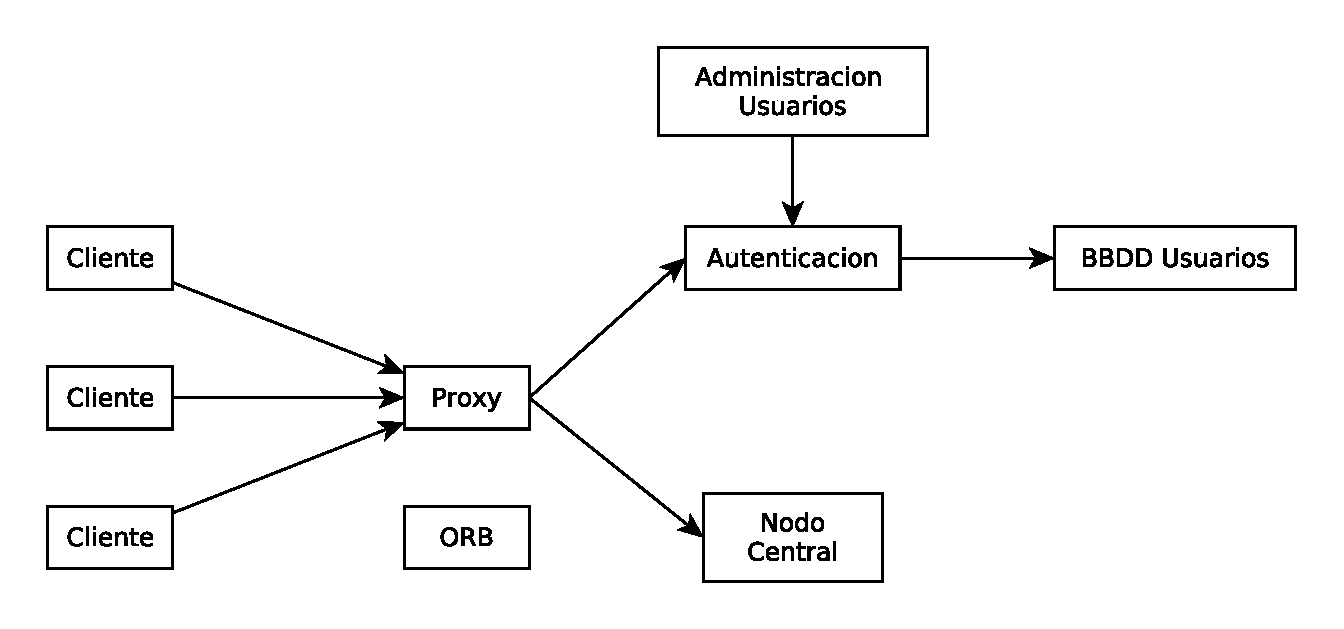
\includegraphics{comun.eps}
		}
		
		Siguiendo el orden cronológico de una petición, el primer nodo a describir es el cliente. Este programa solo tiene un único hilo, y se queda bloqueado. Antes de lanzar el programa java titular, el nodo necesita montar el directorio remoto de las imágenes. Teniendo el directorio remoto montado, el usuario del cliente tiene que copiar de un directorio local al remoto la imagen a la que quiere que se le aplique el filtro. Con la imagen lista, se puede ejecutar el programa. Este muestra al usuario un dialogo por consola en el que se le piden: direccion relativa y nombre de la imagen; el correo de usuario con el que está registrado; su contraseña; y el filtro o lista de filtros que quiere aplicar, separados por comas.
		\linebreak
		
		El programa \textit{Cliente.java} tiene una medida contra fallos, un bucle hasta que el usuario introduzca un nombre de imagen que exista en la carpeta distribuida. El sistema tiene mas medidas contra fallos introducidos por el usuario, pero están implementadas en otros programas. Después de introducir los filtros se crea un hash con la contraseña del usuario, para nunca llegar a enviar esta en claro. Los campos que ha introducido el usuario se envían a Proxy usando CORBA, justificaré esta decisión en la sección de heterogeneidad.
		\linebreak
		 
		El siguiente nodo es Proxy. Este recibe una llamada remota al método \textit{getFiltrado} con los campos del usuario. Los dós primeros, correo y hash de la contraseña son enviados al nodo de autenticación. Este responde con un booleano, si el usuario existe y su contraseña concuerda, o no. En caso negativo, la petición del cliente acaba aqui, devolviendole un \textit{false} como resultado. Si el usuario se autentica, la petición se propaga al nodo central. Durante el diseño pensé que proxy lanzara un hilo por cada petición que le llega, pero en la implementación asumí equivocadamente que CORBA lo generaría automaticamente, cuando necesita ser explícito.
		\linebreak
		
		Es necesario para la comunicación entre Cliente y Proxy que este disponible un broker, este corre en un tercer nodo.
		\linebreak
		
		\hspace*{-1cm}
		\resizebox{1.1\textwidth}{!}{%
			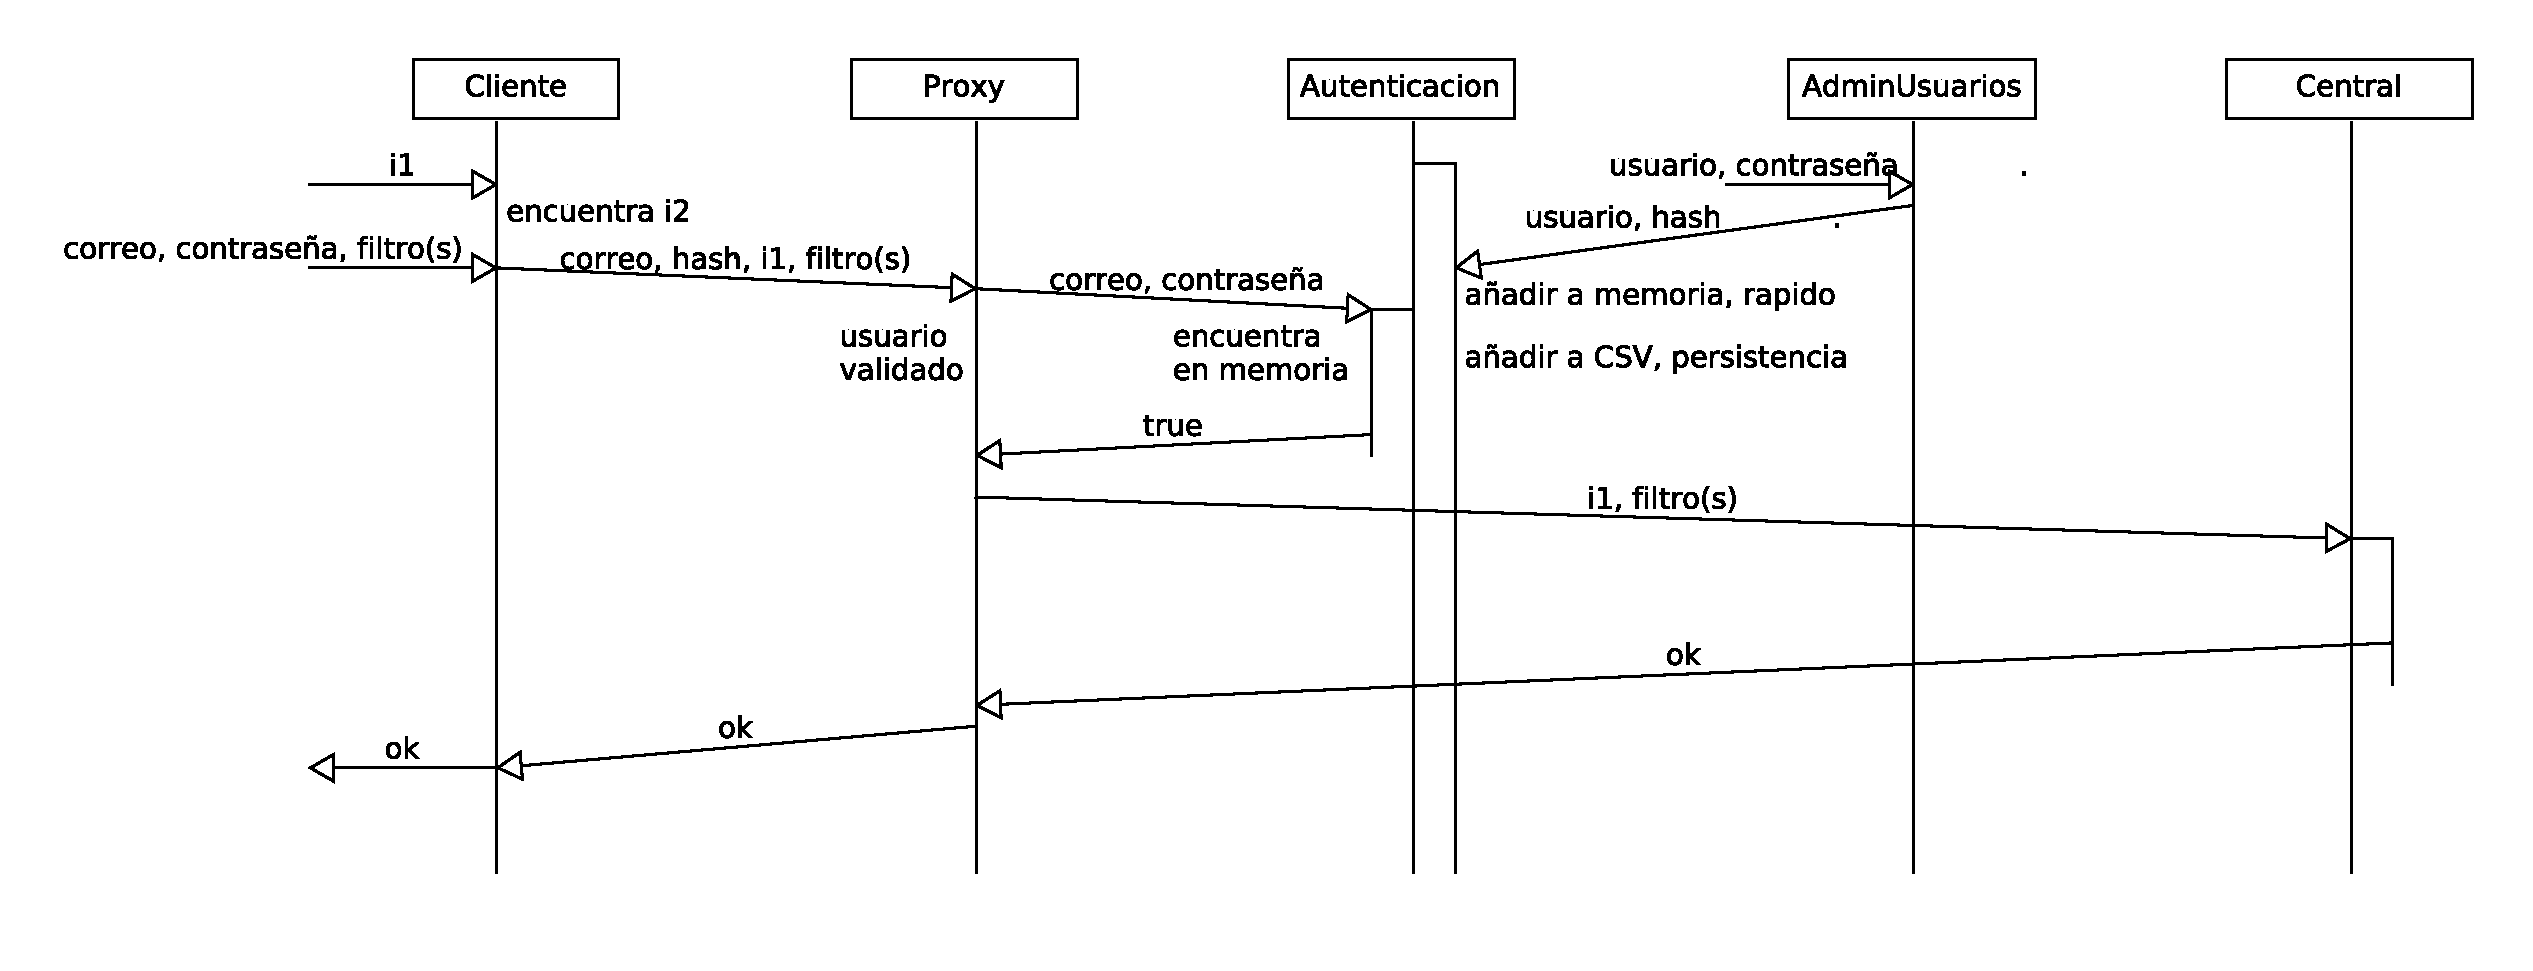
\includegraphics{frontend-seguridad.eps}
		}
		
		La comprobación de los credenciales del usuario es manejada por el nodo de autenticación. A este también se conecta el administrador de usuarios. Al arrancar, carga un CSV en el que están guardados los usuarios y los hash con sus contraseñas. Este programa tiene 2+N hilos, siendo N el numero de peticiónes del proxy simultáneas (esta implementado asumiendo un proxy capaz de varios hilos). En el primer hilo escucha peticiones del proxy, en el segundo del administrador. Las del último son adiciones o eliminaciones de usuarios. Para reflejar los cambios que ordene el administrador rápido, son primero aplicados en el objeto en memoria donde están los credenciales, y después hechos persistir en el CSV.
		\linebreak
		
		El admnistrador de usuarios tiene dos medidas a resaltar. La primera es, igual que el cliente, la conversión de la contraseña a un hash antes de ser enviada. La segunda una protección frente a errores del administrador. Para poder crear un usuario el correo tiene que seguir una expresión regular con el patrón de un correo. Solo se envía a autenticación un usuario para crear después de que el correo introducido cumpla el patrón.
		\linebreak
		
		Los nodos Proxy, Autenticación y Administrador de usuarios se sincronizan al arrancar. Usando el algorítmo de Cristian en un bucle de diez peticiones, se calcula una corrección. Autenticación se sincroniza con Administrador de usuarios y Proxy con Autenticación. Proxy además recibe la corrección de Autenticación respecto a Administrador de usuarios, y guarda la corrección acumulada entre el y el administrador.
		\linebreak
		
		Por último, el nodo central. Este tiene 3+N hilos. El primero es en el que escucha las peticiones de proxy, igual que el nodo de autenticación, esta programado para pasar el proceso de la petición a un trabajador, de manera que sea solo este el que se bloquea durante las siguientes partes de la peticion. El segundo hilo es para escuchar multiservidores dandose de alta. Al arrancar, los multiservidores de tanto el Sistema A como el Sistema B envían un mensaje al nodo central con su dirección y el puerto en el que le van a escuchar. Si un multiservidor se cae, Central lo descubrirá con la siguiente petición de proxy, al hacer un \textit{healthcheck} sobre el. Central elige el multiservidor al que propagar la petición mediante round-robbin. En ambos sistemas el nodo central queda abstraído de como se aplican los filtros, y que anillo los tenga o no. El último hilo que permanece abierto durante el funcionamiento del nodo central es para la escucha del administrador de filtros. Los programas para administrar filtros en el Sistema A y B envían, después de cualquier cambio, la lista con los filtros que están corriendo en anillos (no la lista total de filtros). 
		\linebreak
		
		En Central se detecta el posible error del usuario de introducir un filtro no existente. Aún si envía una lista, y los demás si serían aplicables, la petición es denegada, devolviendo un false a Proxy para que a su vez se lo devuelva a Cliente y el usuario de este lo vuelva a intentar.
		\linebreak
		
		\clearpage
		\subsection{Diferencias y funcionamiento de las variantes}
		Los siguientes diagramas muestran las diferencias en diseño entre el Sistema A (el primer diagrama) y el Sistema B (el segundo). En el Sistema A los multiservidores solo se comunican con un único anillo, pero los nodos de este son capazes de aplicar cualquier filtro de la carpeta remota, a la que todos tienen aceso. 
		\linebreak
		
		\hspace*{-0.5cm}
		\resizebox{1.1\textwidth}{!}{%
			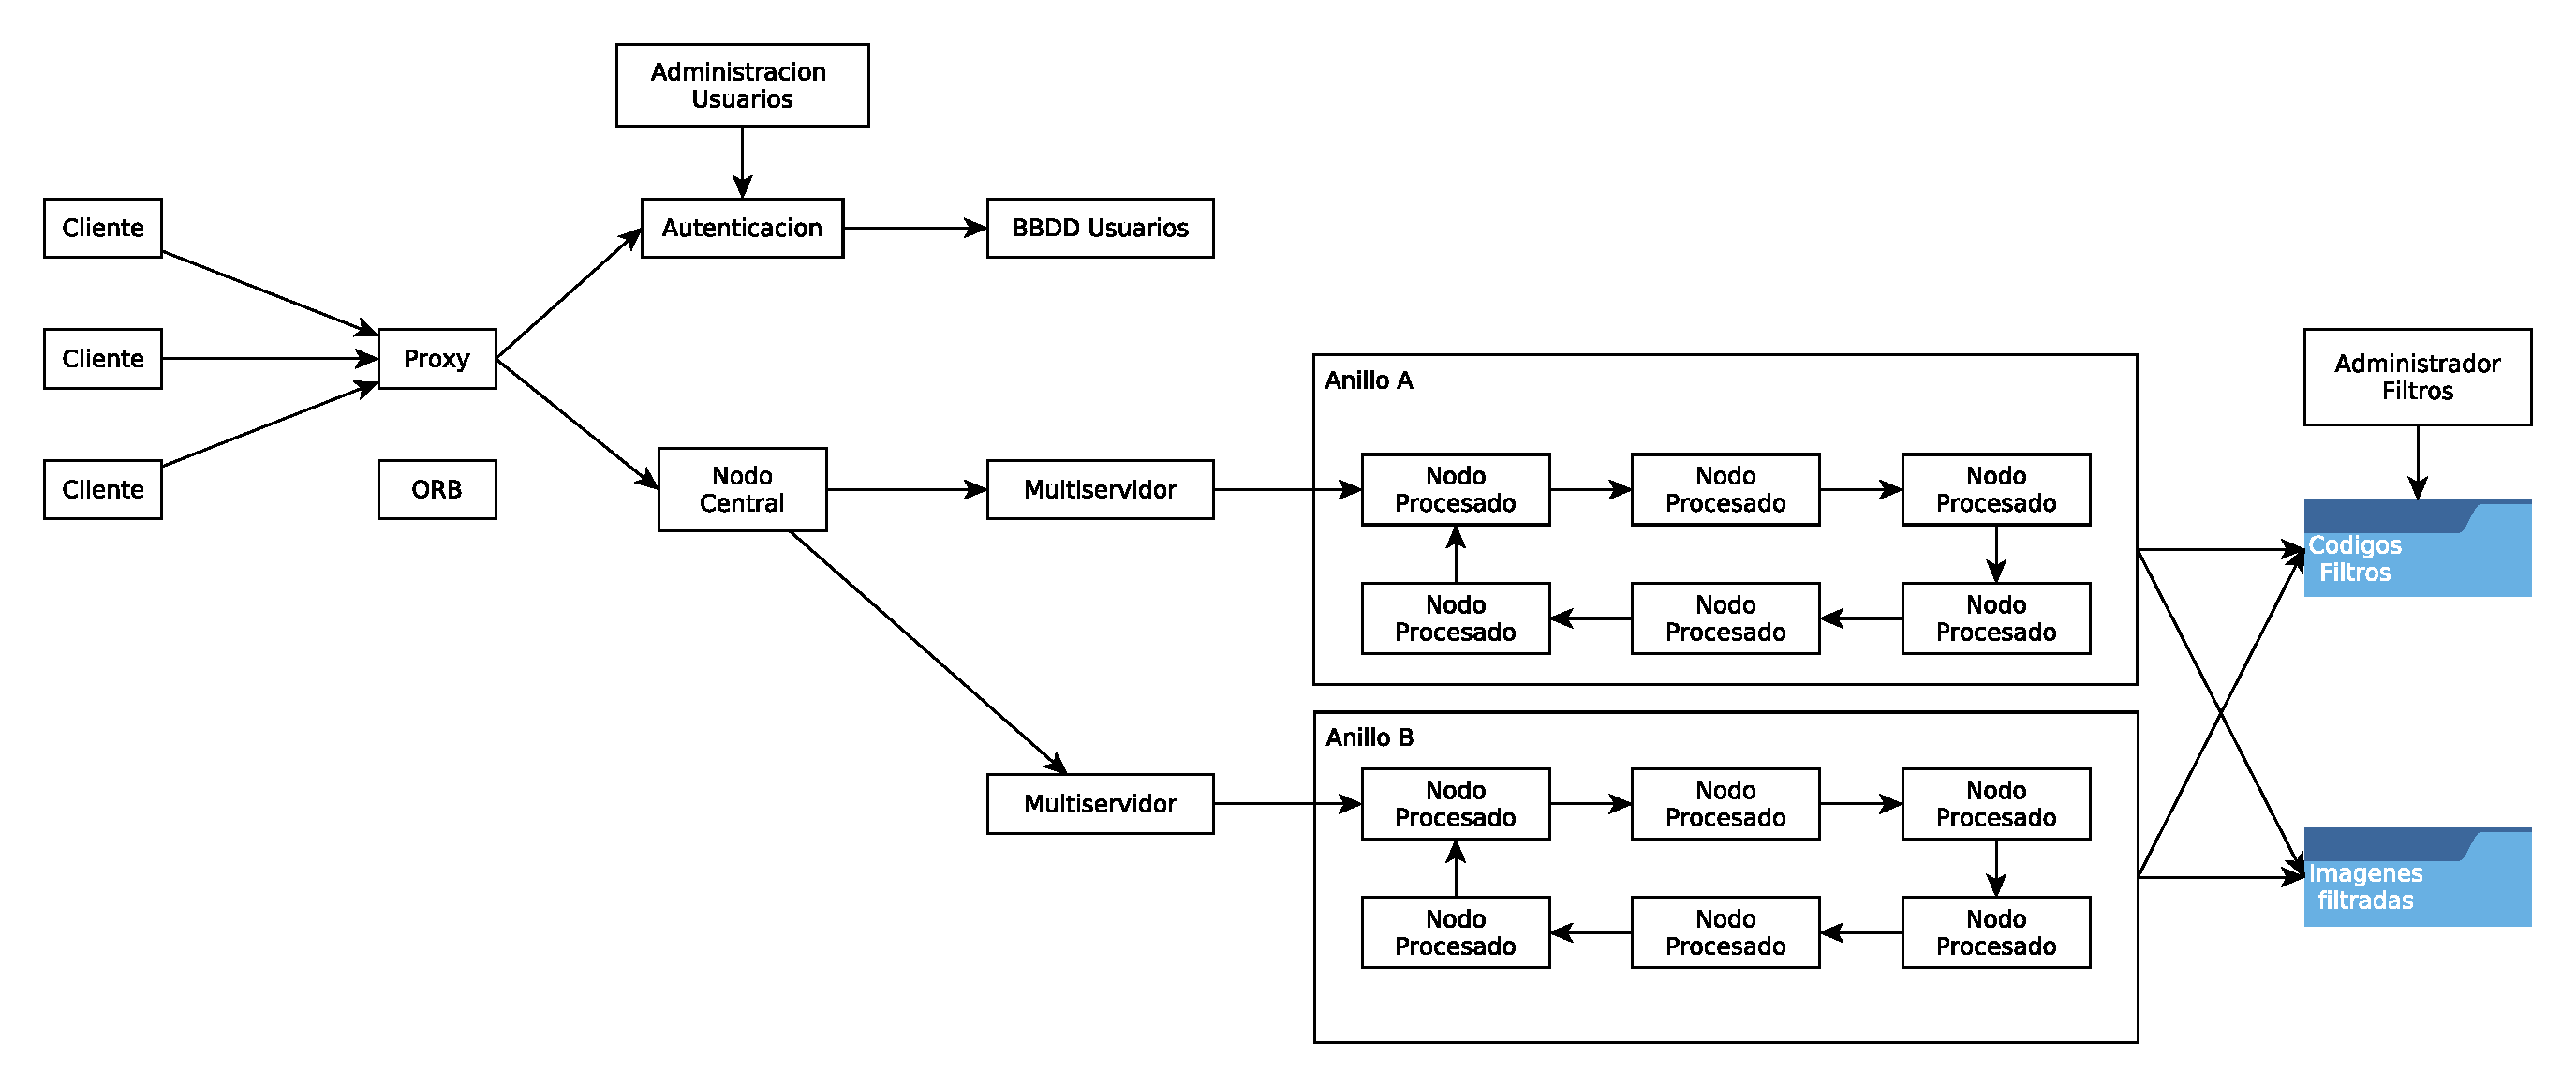
\includegraphics{sistemaA.eps}
		}
		\bigskip

		En el Sistema B, los multiservidores se comunican con todos los anillos, pero cada uno de ellos solo tiene un filtro en cualquier momento dado.
		
		\hspace*{-0.5cm}
		\resizebox{1.1\textwidth}{!}{%
			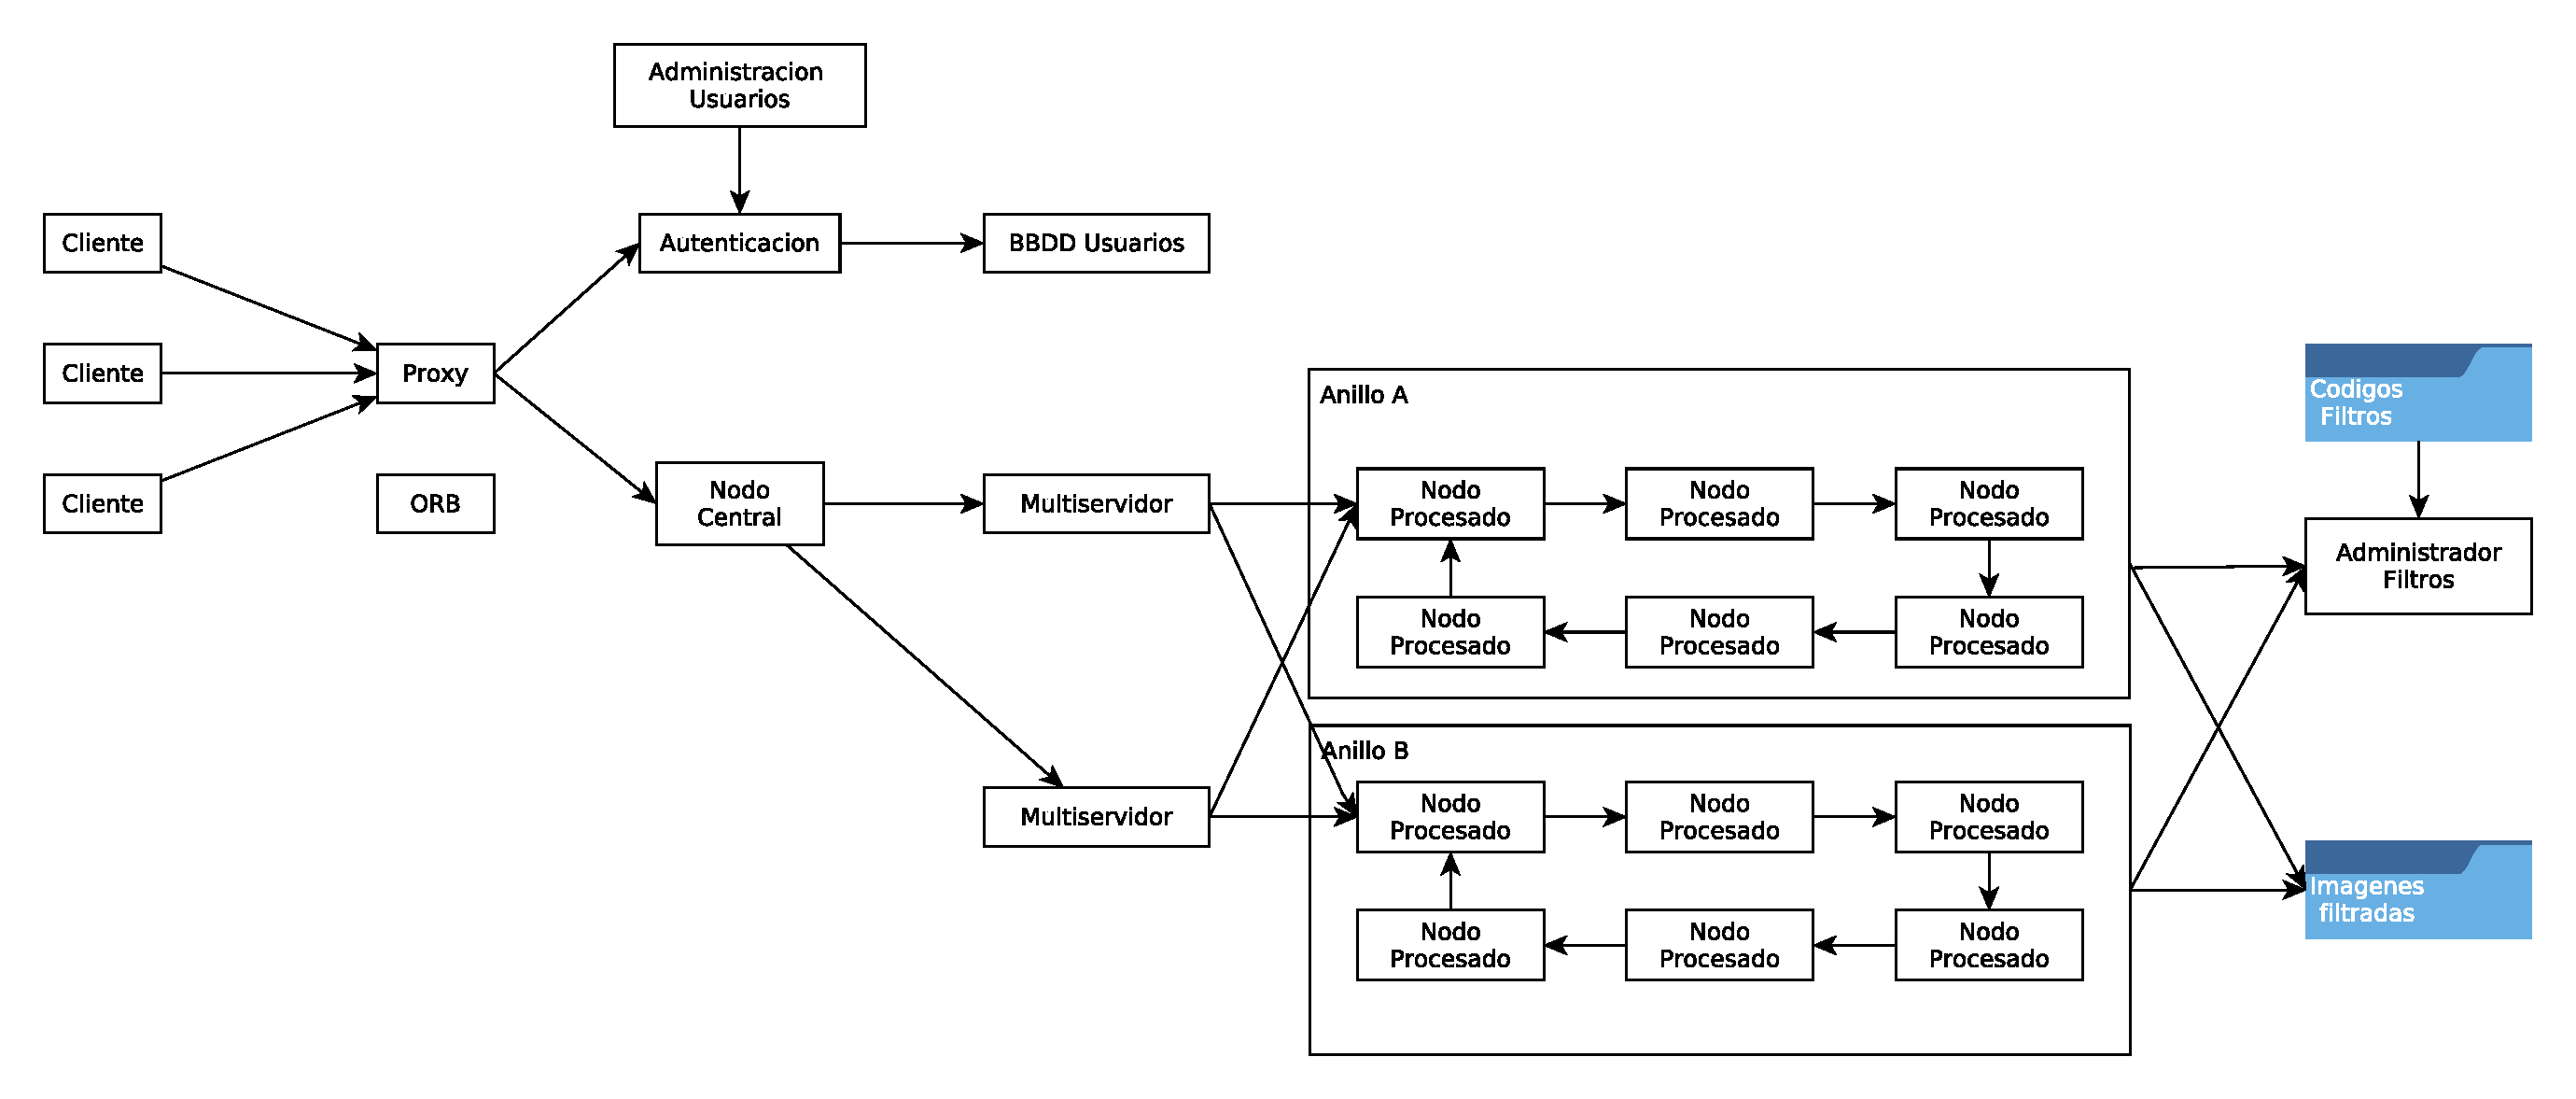
\includegraphics{sistemaB.eps}
		}
		\bigskip
		
		De esta manera, o bien en los nodos de los anillos (Sistema A) o en los multiservidores (Sistema B) se soluciona la disponibilidad de filtros en anillos. Es por esto que es posible un nodo central común a ambos sistemas, ya que no necesita saber los detalles.
			
			\clearpage
			\subsubsection{Sistema A}
			En el Sistema A cada multiservidor tiene un único anillo, pero los nodos de todos los anillos pueden correr todos los filtros de la carpeta compartida. Cada multiservidor tiene un hilo en el que escucha peticiones del central. Las peticiones pueden ser dos, healthcheck o imagen y filtros. Si es la segunda, añade el socket del central y la tarea a una cola. 
			\linebreak
			
			El nodo maestro del anillo hace una inicializacion del testigo pasandolo por todos los nodos intermedios para que añadan en el su disponibilidad (uso de CPU y RAM). Después, se comunica directamente con el multiservidor, el cual con las disponibilidades elije a que nodo le encarga que filtro. El nodo maestro recupera la lista de tareas (parejas de filtro y nodo asignado) y la imagen. Los nodos del anillo aplican el filtro que deban y al llegar el testigo de vuelta al anillo, este repite su comunicacion con el multiservidor. Con esta siguiente interacción, el multiservidor da por aplicados los filtros antes asignados. Al hacerlo, recupera el socket de la cola y envía un ok a Central (para que este lo propague y cierre el hilo de escucha) y retira la petición de la cola.
			\linebreak
			
			\hspace*{-1cm}
			\resizebox{1.1\textwidth}{!}{%
				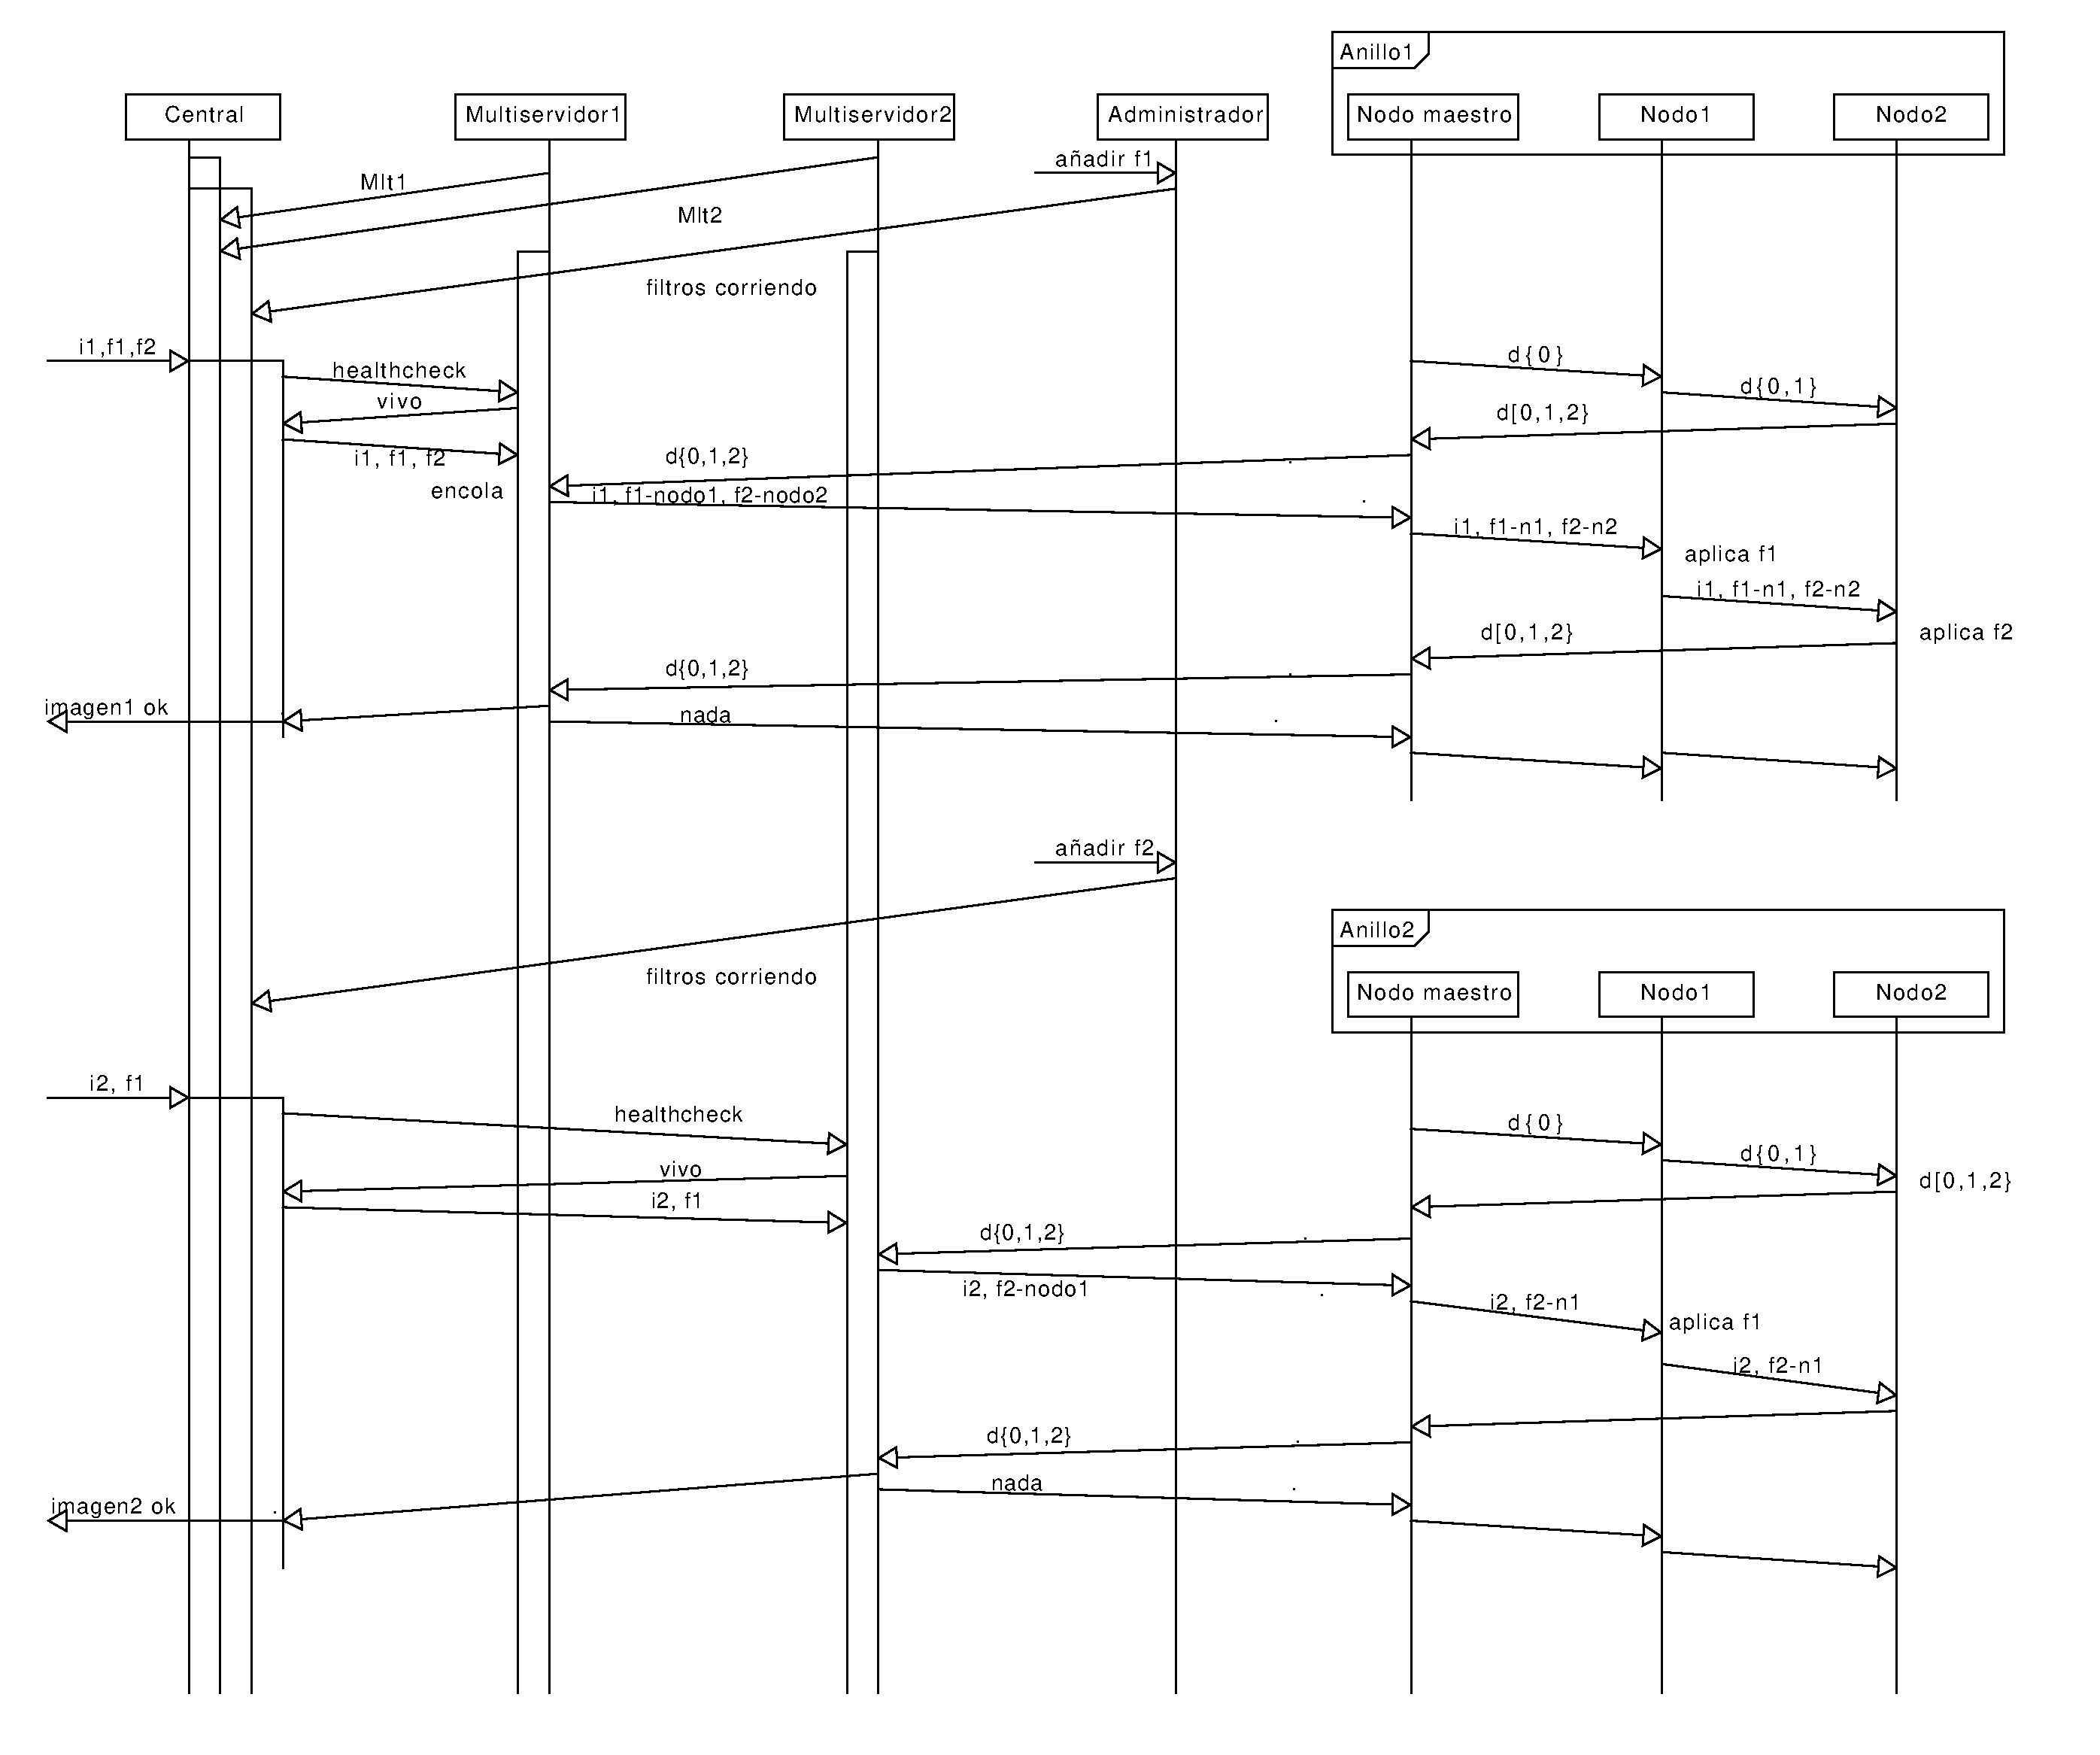
\includegraphics{modAv2.pdf}
			}
			\bigskip
			
			\subsubsection{Sistema B}
			En el Sistema B, a diferencia del A, cualquier multiservidor puede ser contactado por cualquier anillo. Al hacerlo, este busca en su cola peticiones con el filtro del anillo que le ha contactado y devuelve una lista de imagenes que quieren el filtro del anillo. También a diferencia del Sistema A, el Administrador de filtros es ahora contactado directamente por los nodos maestros de cada anillo. Este ya no puede sencillamente avisar a Central de los contenidos de la carpeta remota, porque no la hay. Los maestros preguntan al administrador si su filtro actual es el que tienen asignado, y si no lo es, reciben como mensaje el código del filtro que deberían tener. Al recibirlo, este se añade al testigo. Cada nodo del anillo comprueba si su código es el del testigo, y de no serlo, lo crean en local. Ese entonces se vuelve su fitlro asignado.
			\linebreak
			
			\hspace*{-1cm}
			\resizebox{1.1\textwidth}{!}{%
				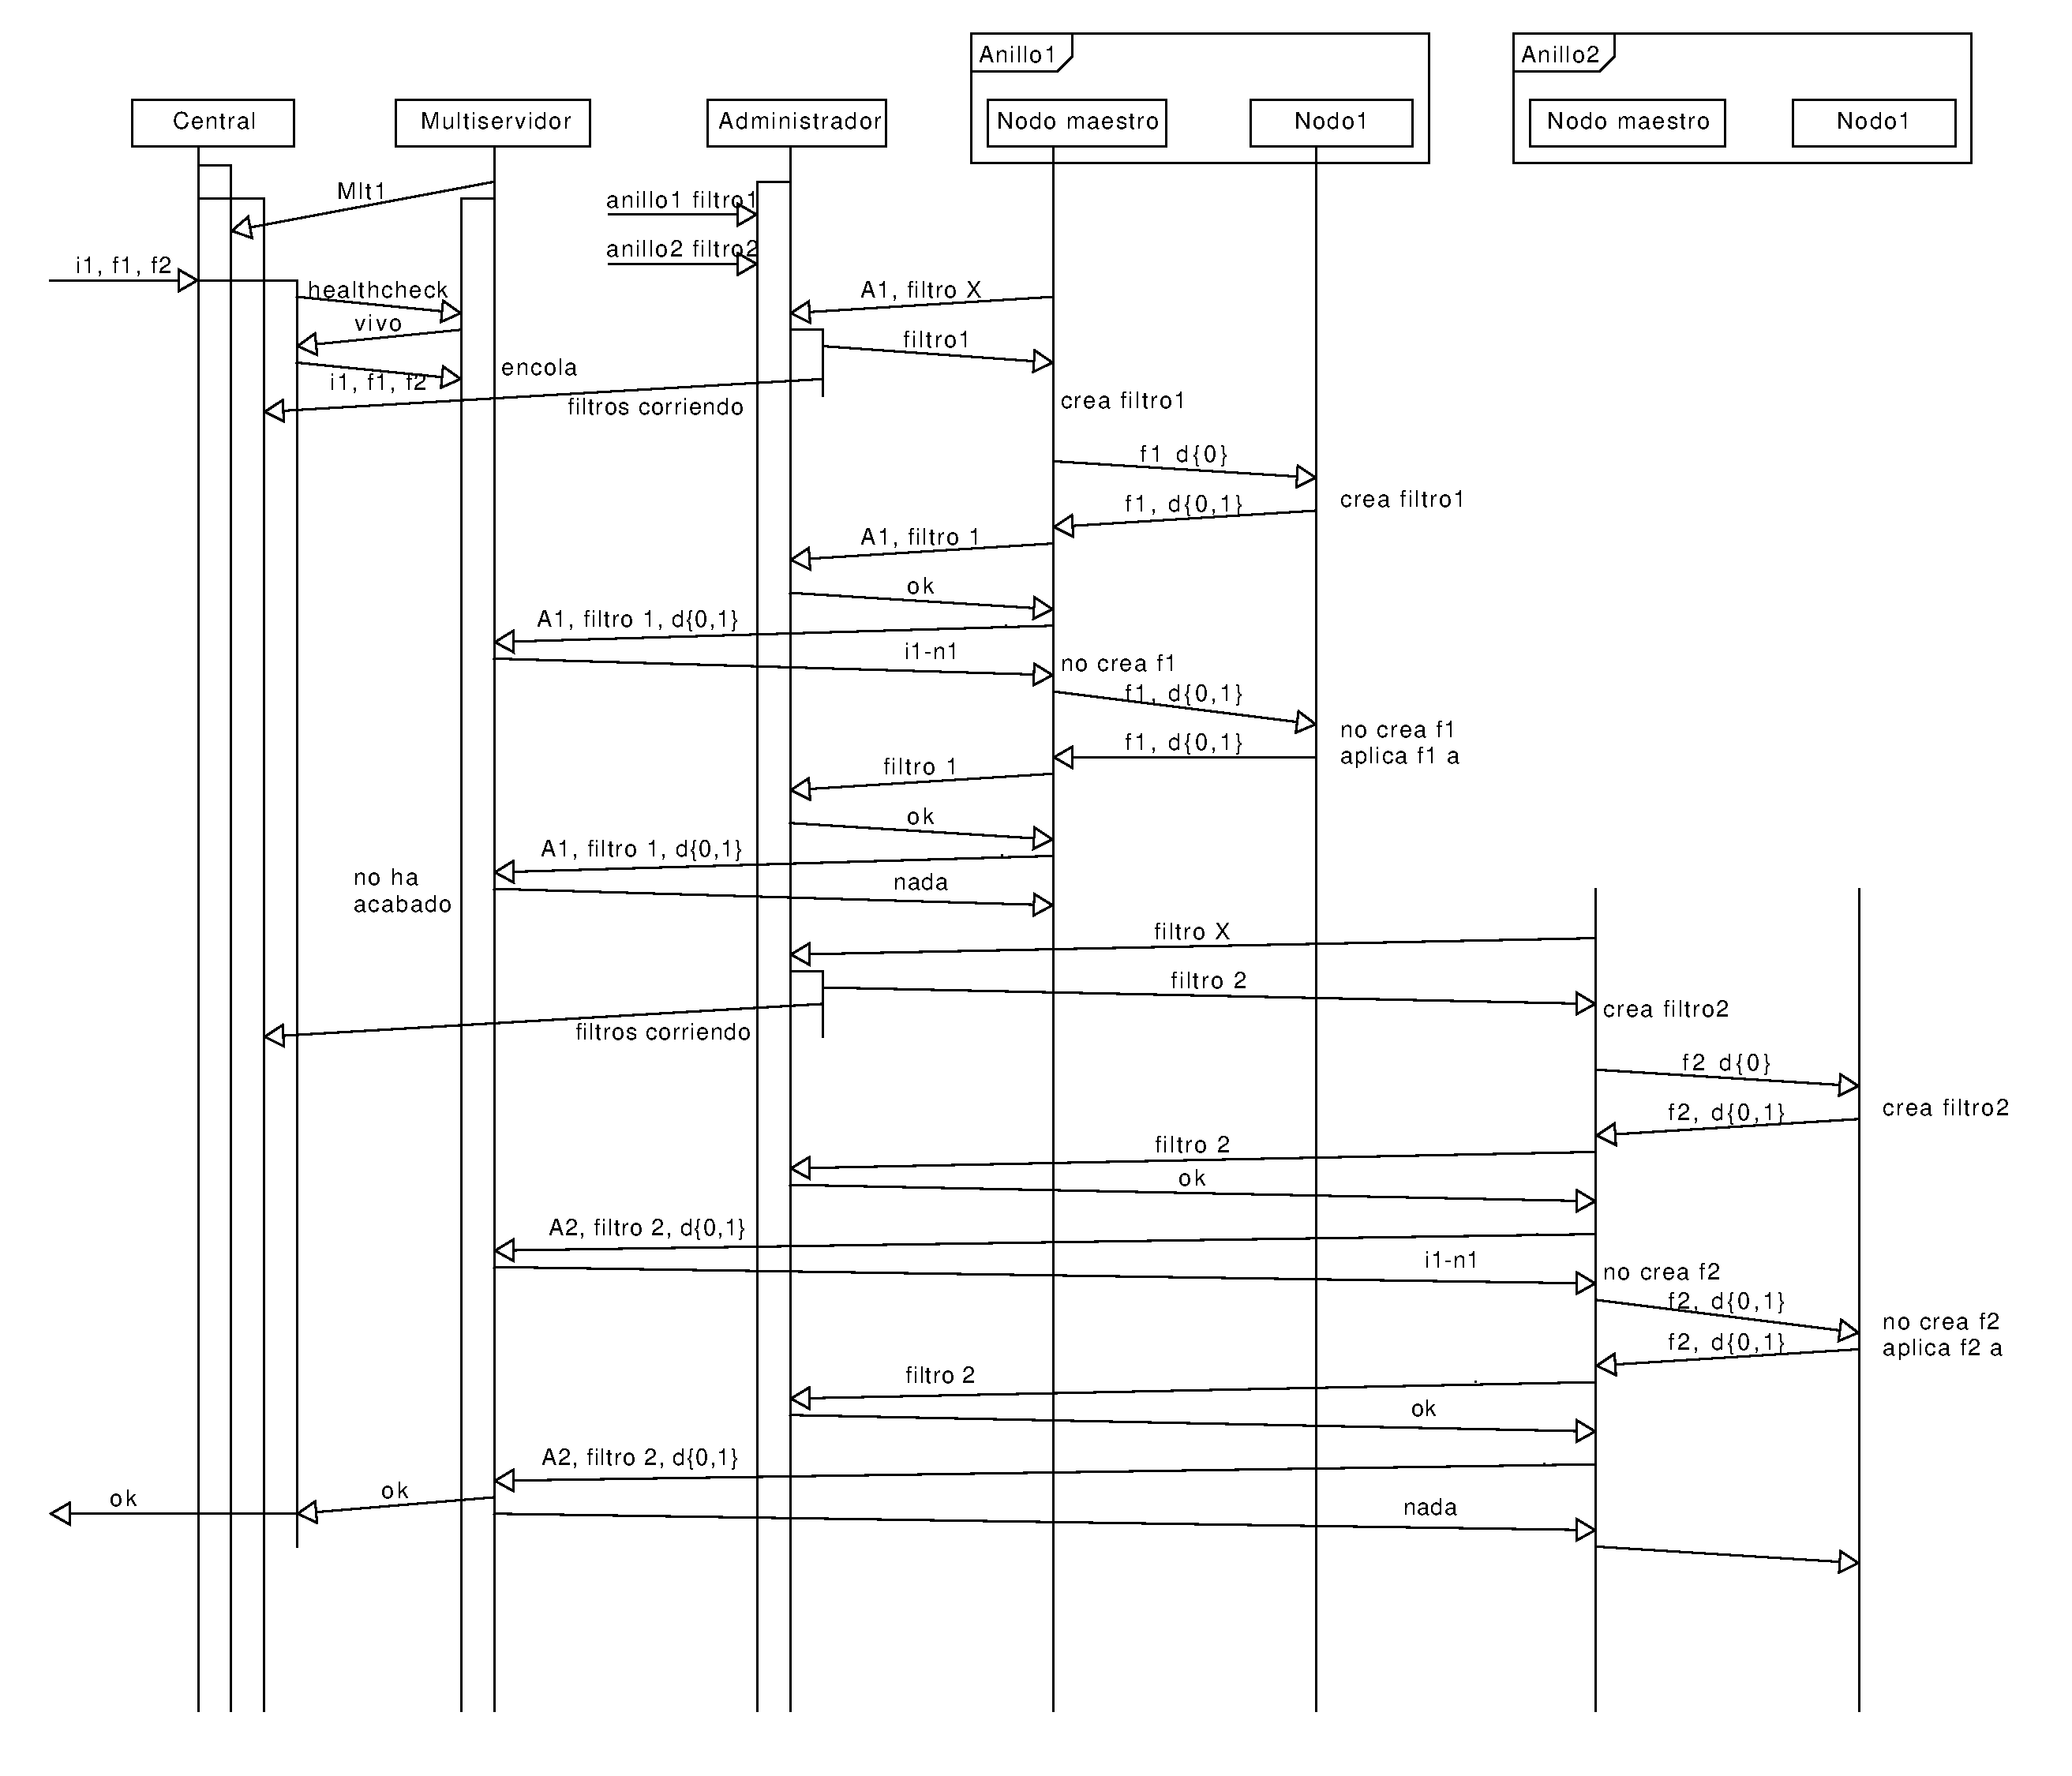
\includegraphics{modB1msv2.pdf}
			}
			
			El diagrma anterior tiene un error, la primera comunicación entre Administrador de Filtros y Central solo envía como filtros corriendo el filtro 1, el único que tendría anillo. La petición que recibe Central sería denegada, porque faltaría el filtro 2. No era posible en un diagrama de dos dimensiones pintar las comunicaciones de los anillos 1 y 2 al mismo tiempo de manera legible. El eje vertical es el tiempo, como en todos los diagramas de pasos de mensajes, pero el anillo 2 y su mensaje de inicialización tendría que estar poco debajo del anillo 1. El anillo 2 se quedaría pasando el testigo entre sus nodos y preguntando al administrador y multiservidor hasta que el anillo 1 acabase, entonces, con la siguiente comunicación al multiservidor, este le devolvería la imagen con la que ha acabado el anillo 1.
			\linebreak
			
			\hspace*{-1cm}
			\resizebox{1.1\textwidth}{!}{%
				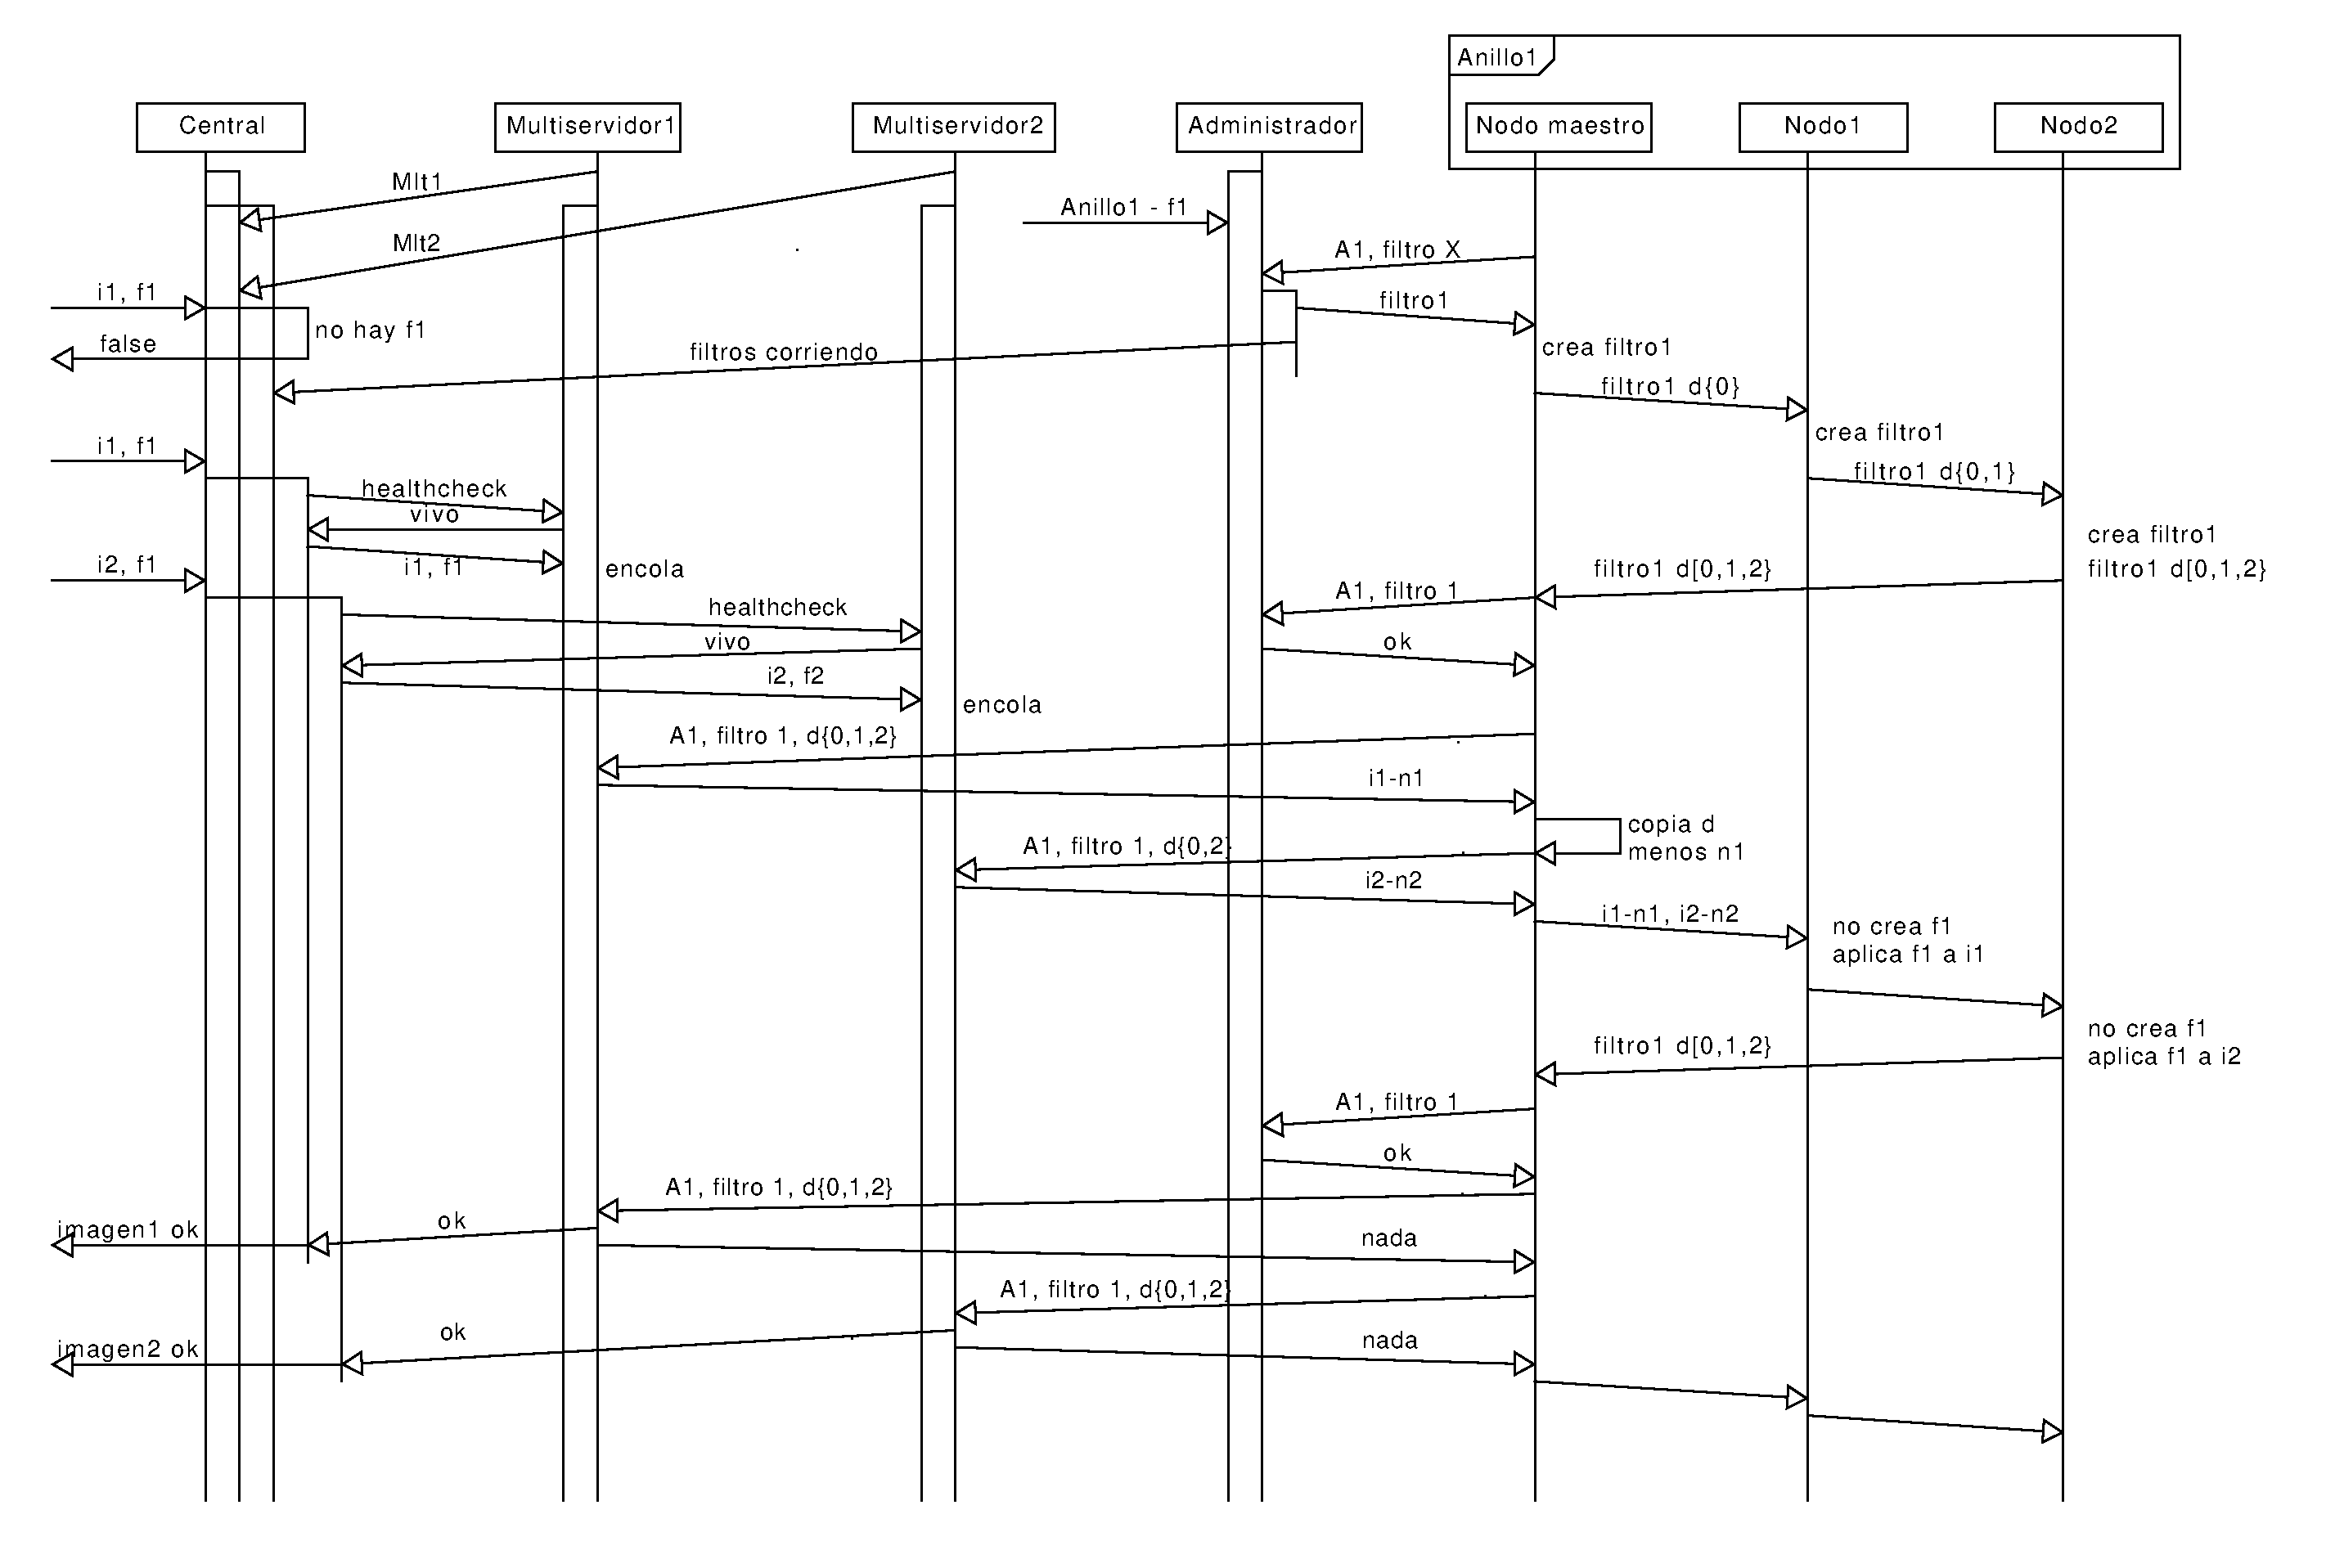
\includegraphics{modB2msv2.pdf}
			}
			
			El primer diagrama muestra dos anillos interactuando con un solo multiservidor, el segundo un solo anillo interactuando con dos multiservidores. Cada multiservidor tiene una cola con peticiones, y las asigna en fución del filtro del anillo y las disponibilidades de los nodos de este. 
	\section{Parámetros de diseño}
	\begin{description}
		\addtolength{\itemindent}{0.5cm}
		\itemsep0em 
		
		\item[Heterogeneidad:] He mencionado que las carpetas remotas están montadas sobre SAMBA. Esta decisión ha sido por la popularidad de este sistema de ficheros, que tiene clientes en la gran mayoría de plataformas. También he mencionado el uso de CORBA en la comunicación entre Cliente y Proxy. Esta otra decisión ha sido para facilitar la escritura de clientes para plataformas distintas en el futuro. De esta manera, esos clientes pueden estar escritos en lenguajes que no sean java, como pasaría si hubiese elegido RMI.
		\item[Extensibilidad:] Con el uso de administradores de filtros, añadir nuevos es trivial, e incluso puede hacerse en tiempo de ejecución.
		\item[Seguridad] 
			\end{description}
			\begin{description}
				\addtolength{\itemindent}{1cm}
				\itemsep0em 
					\item[Confidencialidad:] El único dato que considero necesita estar protegido es la contraseña de los usuarios, que se protege con un hash, enviando así solo este.
					\item[Integridad:] No tengo en cuenta ninguna medida para asegurarla.
					\item[Disponibilidad:] No tengo en cuenta tampoco ninguna protección frente a ataques ni filtrado por IPs.
			\end{description}
		\begin{description}
		\addtolength{\itemindent}{0.5cm}
		\item[Escalabilidad:] Salvo por el problema ya descrito con Proxy, el resto del sistema es escalable. Se pueden añadir mas multiservidores y anillos de manera transparente al usuario, e indolora para el sistema.
		\item[Gestion de fallos] 
		\end{description}
			\begin{description}
				\addtolength{\itemindent}{1cm}
				\itemsep0em 
					\item[Fallos de usuario:] Son detectados a lo largo de la cascada de peticiones y devueltos al usuario para que los corrija.
					\item[Fallos del sistema:] 
					\addtolength{\itemindent}{0.5cm}
					\item[Recuperacion y redundancia:] Un fallo en un nodo de una anillo causa que el anillo entero se apague si no se recupera antes del siguiente testigo. La caida del anillo se puede recuperar volviendolo a lanzar, sin reiniciar mas sistemas. La caída de un multiservidor se puede arreglar reiniciando este y los anillos. Los demás elementos del sistema, de caer, fuerzan el reinicio del sistema entero.
			\end{description}
		\begin{description}
		\addtolength{\itemindent}{0.5cm}
		\item[Concurrencia:] Solo un único usuario puede comunicarse con Proxy.
		\item[Transparencia]
			\end{description}
			\begin{description}
				\addtolength{\itemindent}{1cm}
				\itemsep0em 
					\item[Acceso y ubicación:] El usuario necesita saber la dirección de Proxy y montar la carpeta remota de las imagenes manualmente.
					\item[Concurrencia:] El usuario queda abstraído de la concurrencia del sistema, es manejada por los servidores.
					\item[Replicación:] En ambos sistemas es necesario un reinicio de los anillos si cae un multiservidor, no está manejado en el anillo recuperarse.
					\item[Escalado y prestaciones:] No se tiene que notificar al usuario de escalados, se manejan por los elementos del sistema. Si que se le tiene que avisar de filtros añadidos o retirados por terceros medios.
					\item[Movilidad:] Los administradores de filtros permiten añadir y quitar los filtros sin derribar el sistema.
	\end{description}
	\section{Objetivos cumplidos}
	El enunciado especifica ocho puntos básicos necesarios para alcanzar el aprovado. Estos son: el correcto funcionamiento de los Sistema A y B; uso de serialización en el sistema; uso de RMI o CORBA en alguna de las comunicaciones; una definicion justificada de los multiservidores; sincronización del sistema; el uso de un sistema de archivos distribuidos para el almacenamiento de las imagenes en el Sistema A y B; el uso de un sistema de archivos distribuidos en el Sistema A para los filtros; y un fichero en cada nodo donde se refleje el uso que recibe. He podido implementar todos por completo, salvo por la sincronización de los nodos. Solo he tenido tiempo para implementar sincronización entre algunos de ellos, explicaré por que no lo he hecho para todo el sistema, como lo haría para el sistema entero, y por que he elegido los que he hecho para esta implementacion reducida en la siguiente sección.
	\linebreak
		
	Se manejan los accesos concurrentes a recursos compartidos usando \textit(synchronized) de java y por exclusión mutua con los testigos de los anillos. El sistema tiene varias redundancias a errores.
\end{flushleft}
\end{document}